\documentclass[t,usenames,dvipsnames]{beamer}
\usetheme{Copenhagen}
\setbeamertemplate{headline}{} % remove toc from headers
\beamertemplatenavigationsymbolsempty

\usepackage{amsmath, tikz, xcolor}
\usetikzlibrary{arrows.meta, calc}

\title{Circles}
\author{}
\date{}

\AtBeginSection[]
{
  \begin{frame}
    \frametitle{Objectives}
    \tableofcontents[currentsection]
  \end{frame}
}

\begin{document}

\begin{frame}
    \titlepage
\end{frame}

\section{Write the Standard Form of the Equation of a Circle.}

\begin{frame}{}
A \alert{circle} is the set of all points $(x, y)$ in the plane whose distance (the \textit{radius}) from a fixed point (the \textit{center}) is constant.   \newline\\

\begin{center}
    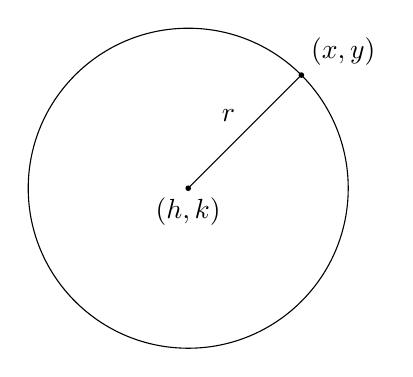
\begin{tikzpicture}[scale=0.8]
    \draw (0,0) circle (1in);
    \draw [fill=black] (0,0) circle (1pt) node [below] {$(h, k)$};
    \draw (0,0) -- (45:1in) node [above right] {$(x,y)$};
    \draw [fill=black] (45:1in) circle (1pt);
    \node at (45:0.5in) [above left] {$r$};
    \end{tikzpicture}
\end{center}    
\pause
The equation can be found by incorporating the distance formula (Pythagorean Theorem):
\[
r^2 = (x-h)^2 + (y-k)^2
\]
\end{frame}

\begin{frame}{Example 1}
Write the standard from of the equation of a circle with center $(-2, 3)$ and radius 5.
\begin{align*}
    \onslide<2->{(x-(-2))^2 + (y-3)^2 = 5^2} \\[10pt]
    \onslide<3->{(x+2)^2 + (y-3)^2 = 25} \\
\end{align*}
\end{frame}

\begin{frame}{Example 2}
Write the standard form of the equation of a circle which has $(-1, 3)$ and $(2, 4)$ as the endpoints of the diameter.  \newline\\ \pause

The center is the \alert{midpoint} of the endpoints of the diameter:
\begin{align*}
    \onslide<3->{h = \frac{-1+2}{2} \quad & \quad k = \frac{3+4}{2}} \\[10pt]
    \onslide<4->{h = \frac{1}{2} \quad & \quad k = \frac{7}{2}} \\
\end{align*}
\end{frame}

\begin{frame}{Example 2}
\onslide<1->{The radius is half the length of the diameter.}
\begin{align*}
    \onslide<2->{d &= \sqrt{(2-(-1))^2 + (4-3)^2}} \\[10pt]
    \onslide<3->{&= \sqrt{10}} \\[10pt]
    \onslide<4->{r &= \frac{\sqrt{10}}{2}} \\[8pt]
\end{align*}
\end{frame}

\begin{frame}{Example 2}
$h = \frac{1}{2} \qquad k = \frac{7}{2} \qquad r = \frac{\sqrt{10}}{2}$
\begin{align*}
\onslide<1->{\left(x-\frac{1}{2}\right)^2 + \left(y-\frac{7}{2}\right)^2 &= \left(\frac{\sqrt{10}}{2}\right)^2}  \\[10pt]
\onslide<2->{\left(x-\frac{1}{2}\right)^2 + \left(y-\frac{7}{2}\right)^2 &= \frac{10}{4}}    \\[10pt]
\onslide<2->{\left(x-\frac{1}{2}\right)^2 + \left(y-\frac{7}{2}\right)^2 &= \frac{5}{2}} \\
\end{align*}
\end{frame}

\section{Find the Center and Radius of a Circle.}

\begin{frame}{Example 3}
Find the center and radius of $(x+2)^2 + (y-1)^2 = 4$.   \newline\\ \pause

$h = -2 \qquad k = 1$   \pause  \newline\\

Center: $(-2, 1)$   \pause  

\begin{align*}
    \onslide<4->{r^2 &= 4} \\
    \onslide<5->{r & = 2} 
\end{align*}

\onslide<6->{Radius: 2}
\end{frame}

\begin{frame}{Finding Center and Radius When Not in Standard Form}
We can use the techniques of finding vertices of parabolas to find the center and radius of a circle not in standard form.   \newline\\    \pause 

\begin{enumerate}
    \item Move any constants to the other side of the equation. \newline\\ \pause
    \item Find the $x$-coordinates of the vertices of the $x$ and $y$ terms. These are your $h$ and $k$, respectively.    \newline\\ \pause
    \begin{itemize}
        \item Use $x$'s as the variable when finding the vertex for the $y$'s parabola.  \newline\\ \pause
    \end{itemize}
    \item Add the absolute value of the $y$-coordinates of the vertices to the right side.
\end{enumerate}
\end{frame}

\begin{frame}{Example 4a}
Find the center and radius of each. \newline\\
(a) \quad $3x^2 - 6x + 3y^2 +4y - 4 = 0$
\begin{align*}
    \onslide<2->{{\color{red}3x^2-6x} + {\color{blue}3y^2 + 4y} &= 4} 
\end{align*}
\begin{minipage}{0.4\textwidth}
\onslide<3->{
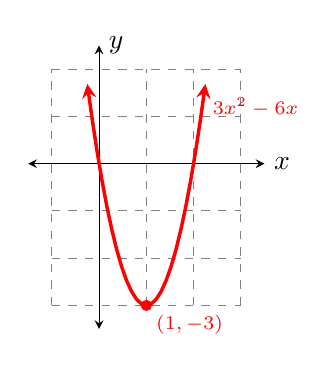
\begin{tikzpicture}[scale=0.6]
\draw[dashed,gray] (-1,-3) grid (3,2);
\draw[<->,>=stealth] (-1.5,0) -- (3.5,0) node [right] {$x$};
\draw[<->,>=stealth] (0,-3.5) -- (0,2.5) node [right] {$y$};
\draw[<->,>=stealth,color=red,line width=1.25,domain=-0.25:2.25] plot (\x,{3*\x*\x - 6*\x});
\draw[color=red,fill=red] (1,-3) circle (3pt) node [below right] {\scriptsize $(1,-3)$};
\node[color=red, anchor=west] at (2.2,1.2) {\scriptsize $3x^2-6x$};
\end{tikzpicture}
}
\end{minipage}
\hspace{0.25cm}
\onslide<4->{
\begin{minipage}{0.4\textwidth}
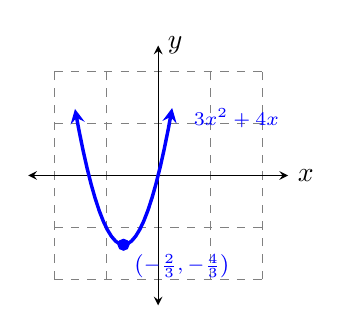
\begin{tikzpicture}[scale=0.66]
\draw[dashed,gray] (-2,-2) grid (2,2);
\draw[<->,>=stealth] (-2.5,0) -- (2.5,0) node [right] {$x$};
\draw[<->,>=stealth] (0,-2.5) -- (0,2.5) node [right] {$y$};
\draw[<->,>=stealth,color=blue,line width=1.25,domain=-1.6:0.27] plot (\x,{3*\x*\x + 4*\x});
\draw[color=blue,fill=blue] (-0.667,-1.333) circle (3pt) node [below right] {\scriptsize $\left(-\frac{2}{3},-\frac{4}{3}\right)$};
\node[color=blue, anchor=west] at (0.5,1.1) {\scriptsize $3x^2+4x$};
\end{tikzpicture}
\end{minipage}
}
\end{frame}

\begin{frame}{Example 4a}
    \begin{align*}
    {\color{red}3(x-1)^2} + {\color{blue}3\left(y+\frac{2}{3}\right)^2} &= 4 + {\color{red}|-3|} + {\color{blue}\left|-\frac{4}{3}\right|} \\[10pt]
    \onslide<2->{3\left(x-1\right)^2 + 3\left(y+\frac{2}{3}\right)^2 &= \frac{25}{3}} \\[10pt]
    \onslide<3->{(x-1)^2 + \left(y+\frac{2}{3}\right)^2 &= \frac{25}{9}} \\
    \end{align*}
    
\onslide<4->{Center: $\left(1, -\frac{2}{3}\right)$} \qquad 
\onslide<5->{Radius: $\sqrt{\frac{25}{9}} = \frac{5}{3}$}
\end{frame}

\begin{frame}{Example 4b}
(b) \quad $2x^2 + 5x + 2y^2 - 8y + 1 = 0$
\begin{align*}
\onslide<2->{{\color{red}2x^2+5x} + {\color{blue}2y^2-8y} &= -1}
\end{align*}
\begin{minipage}{0.5\textwidth}
\onslide<3->{
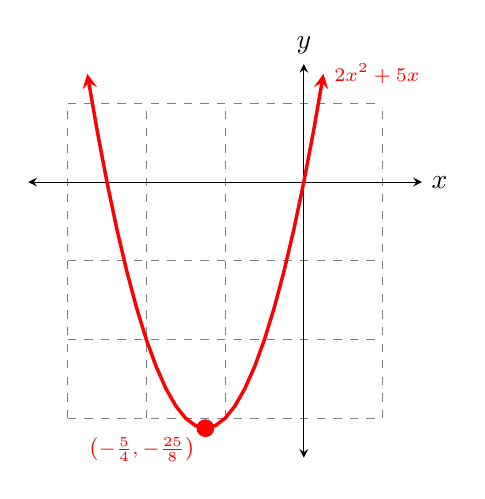
\begin{tikzpicture}
\draw[dashed, gray] (-3,-3) grid (1,1);
\draw[<->,>=stealth] (-3.5,0) -- (1.5,0) node [right] {$x$};
\draw[<->,>=stealth] (0,-3.5) -- (0,1.5) node [above] {$y$};
\draw[<->,>=stealth,color=red,line width=1.25,domain=-2.75:0.25] plot (\x, {2*\x*\x + 5*\x}) node [right] {\scriptsize $2x^2+5x$};
\draw[color=red,fill=red] (-1.25,-3.125) circle (3pt);
\node[color=red, anchor=north east] at (-1.25,-3.125) {\scriptsize $\left(-\frac{5}{4}, -\frac{25}{8}\right)$};
% \node[color=red, anchor=west] at (0,-0.5) {\scriptsize $2x^2+5x$};
\end{tikzpicture} }
\end{minipage}
\hspace{0.25cm}
\onslide<4->{
\begin{minipage}{0.4\textwidth}
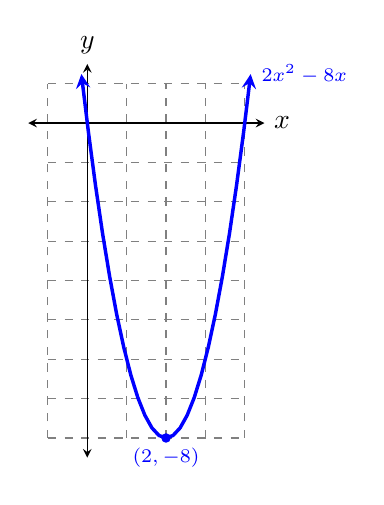
\begin{tikzpicture}[scale=0.5]
\draw[dashed,gray] (-1,-8) grid (4,1);
\draw[<->,>=stealth] (-1.5,0) -- (4.5,0) node [right] {$x$};
\draw[<->,>=stealth,] (0,-8.5) -- (0,1.5) node [above] {$y$};
\draw[<->,>=stealth,color=blue,line width=1.25,domain=-0.15:4.15] plot (\x, {2*\x*\x - 8*\x}) node [right] {\scriptsize $2x^2-8x$};
\draw[color=blue,fill=blue] (2,-8) circle (3pt) node [below] {\scriptsize $(2,-8)$};
\end{tikzpicture}
\end{minipage}
}
\end{frame}

\begin{frame}{Example 4b}
\begin{align*}
    {\color{red}2\left(x+\frac{5}{4}\right)^2} + {\color{blue}2\left(y-2\right)^2} &= -1 + {\color{red}\left|-\frac{25}{8}\right|} + {\color{blue}|-8|} \\[8pt]
    \onslide<2->{2\left(x+\frac{5}{4}\right)^2 + 2(y-2)^2 &= \frac{81}{8}} \\[8pt]
    \onslide<3->{\left(x+\frac{5}{4}\right)^2 + (y-2)^2 &= \frac{81}{16}}   \\
\end{align*}

\onslide<4->{Center: $\left(-\frac{5}{4}, 2\right)$} \qquad
\onslide<5->{Radius: $\sqrt{\frac{81}{16}} = \frac{9}{4}$}
\end{frame}

\end{document}
